%&../settings/preamble.main

\ifsubfile
\pagestyle{plain}
\setcounter{chapter}{1}

% arara: pdflatex: { options: ["--output-directory=../build"], draft: yes, synctex: no }
% arara: pdflatex: { options: ["--output-directory=../build"], synctex: no }
\begin{document}
\fi
\chapter{Analisi di algoritmi}

\section{Introduzione}

Il nostro obiettivo è \emph{stimare la complessità in tempo} degli algoritmi.
Dovremmo stimare anche quella in spazio, ma la complessità in spazio dipende da quella in tempo.
Daremo delle definizioni, parleremo di modelli di calcolo, faremo qualche esempio di valutazione precisa e introdurremo una notazione.
Faremo tutto questo per stimare il tempo per un dato input, per stimare il più grande input gestibile in tempi ragionevoli, per avere un metodo di confronto fra diversi algoritmi ed in particolare per ottimizzare le parti più importanti di un particolare algoritmo.

\subsection*{Definizione di complessità}

La complessità viene definita come una funzione che, data la dimensione dell'input, restituisce il tempo, considerato come un valore intero.

Come definiamo quindi la dimensione dell'input?
Come misuriamo il tempo?

\section{Valutare la dimensione dell'input}

Esistono due criteri per valutare la dimensione dell'input:
\begin{enumerate}
	\item il criterio di \textbf{costo logaritmico}: dove la dimensione dell'input è il numero di bit necessari per rappresentarlo (un esempio è la moltiplicazione di numeri binari, lunghi \(n\) bit);
	\item il criterio di \textbf{costo uniforme}: dove la dimensione dell'input è il numero di elementi di cui è costituito (un esempio è la ricerca del minimo in un vettote di \(n\) elementi).
\end{enumerate}

Ad esempio, consideriamo \(n\) interi rappresentati tramite \(32\) bit.
Nel criterio di costo uniforme hanno un costo pari ad \(n\), mentre nel criterio di costo logaritmico hanno un costo pari a \(32n\).
In molti casi, infatti, possiamo assumere che gli \enquote{elementi} siano rappresentati da un numero costante di bit e che le due misure coincidano a meno di una costante moltiplicativa.

Il criterio che abbiamo utilizzato fin'ora --- e che useremo d'ora in poi --- è il criterio del costo uniforme (in casi particolari utilizzeremo il criterio di costo logaritmico).

\section{Misurare il tempo}

Consideriamo un'istruzione come elementare se può essere eseguita in tempo \enquote{costante} dal processore.
Facciamo qualche esempio:
\begin{itemize}
	\item \texttt{a *= 2} effettua un'operazione di \foreign{shift}, è una singola operazione macchina;
	\item \texttt{Math.cos(d)} può essere considerata come un'operazione elementare;
	\item \texttt{min(A, n)} \underline{non} può essere considerata un'operazione elementare poiché si richiede il minimo di un vettore \emph{arbitrariamente lungo}.
\end{itemize}

Ma allora come possiamo distinguere in maniera precisa un'operazione elementare da una che non lo è?

Per farlo abbiamo bisogno di un modello di calcolo, ossia una rappresentazione astratta di un calcolatore.
Il quale deve:
\begin{enumerate}
	\item permettere di nascondere i dettagli (tramite \emph{astrazione})
	\item riflettere la situazione reale (\emph{realismo})
	\item permettere di trarre conclusioni \enquote{formali} sul contesto.
\end{enumerate}
La pagina di Wikipedia dei modelli di calcolo presenta centinaia di modelli di calcolo diversi.
La macchina di Turing ne è un esempio.
\`{E} una macchina ideale che manipola, seconodo un insieme prefissato di regole, i dati contenuti su un nastro di lunghezza infinita.
Ad ogni passo, la Macchina di Turing:
\begin{enumerate}
	\item legge il simbolo sotto la testina;
	\item modifica il proprio stato interno;
	\item scrive il nuovo simbolo nella cella;
	\item muove la testina a destra o a sinistra.
\end{enumerate}
Nel corso di laurea magistrale è possibile approfondire questo aspetto, per i nostri scopi questa è una trattazione dell'argomento troppo a basso livello.

Noi utilizzeremo il modello di calcolo RAM, che sta per Random Access Machine, ossia una macchina che ha una quantità infinita di celle (di dimensione finita) e accesso in tempo costante indipendentemente dalla posizione (diversamente da ciò che avviene nei nastri); un singolo processore con un set di istruzioni simile a quelli reali, i cui costi di esecuzione sono uniformi e ininfluenti ai fini della valutazione (faremo un esempio più avanti).

\subsection{Calcolo della complessità}

Proviamo a calcolare la complessità dell'algoritmo che ricerca il minimo.

\begin{algorithm}[H]
\caption*{Calcolo della complessità della ricerca del minimo in un vettore}

\BlankLine
% \tcp{calcola il minimo di un vettore arbitrariamente lungo}
\prototype{\minFunction{\Item{} A, \Int n}}{

	\vspace{-5pt}
	\Rem*[r]{\costo*{Costo}[\# Volte]}

	% \BlankLine
	\Item \(min \Assign A[i]\)\costo{c_1}[1]

	\BlankLine
	\From(\costo{c_2}[n]){\(i \Assign 2\) \DownTo \(n\)}{

		\BlankLine
		\If(\costo{c_3}[n-1]){\(A[i] < min\)}{
			\(min \Assign A[i] \)\costo{c_4}[n-1]
		}
	}

	\BlankLine
	\Return \(min\)\costo{c_5}[1]
}
\end{algorithm}

\vspace{-15pt}% NOTE aggiustamento locale della spaziatura sotto l'algoritmo
\paragraph{Ragionamento sul calcolo della complessità}
L'assegnazione del minimo parziale viene eseguita solo una volta.
Il ciclo viene eseguito \(n\) volte.
Considerando \emph{il caso pessimo}, ovvero un vettore ordinato in modo decrescente, il controllo \(A[i] < min\) viene eseguito \(n-1\) volte in quanto ogni elemento che incontreremo sarà minore del precedente.
Infine l'istruzione di ritorno viene eseguita una volta sola.

Bisogna tenere ben a mente che:
\begin{itemize}
	\item ogni istruzione richiede un tempo costante per essere eseguita e
	\item viene eseguita un certo numero di volte, dipendente da \(n\) e
	\item la costante è potenzialmente diversa da istruzione a istruzione.
\end{itemize}

Sommando tutte le costanti il costo totale risultante è:
\[\begin{WithArrows}
T(n)	&= c_1 + c_2n + c_3(n-1) + c_4(n-1) + c_5 \Arrow{raccogliamo}\\
		&= (c_2+c_3+c_4)n + (c_1+c_5-c_3-c_4) \Arrow{semplifichiamo}\\
		&= an+b
\end{WithArrows}\]

Possiamo quindi notare che le costanti vanno a semplificarsi nei parametri \(a\) e \(b\).
% Le singole operazioni hanno dei costi dipendenti da \(n\)

Proviamo a calcolare la complessità dell'algoritmo che ricerca un numero intero all'interno di un vettore ordinato.

\begin{algorithm}[H]
\caption*{Calcolo della complessità della ricerca di un numero intero in un vettore ordinato}

\BlankLine
% \tcp{effettua una ricerca binaria su un vettore}
\prototype{\binarySearch{\Item{} A, \Item v, \Int i, \Int j}}{

	\vspace{-5pt}
	\Rem*[r]{\costo*{Costo}[\# \(i > j\)][\# \(i \leqslant j\)]}

	% \BlankLine
	\eIf(\costo{c_1}[1][1]){\(i > j\)}{
		\Return \(0\)\costo{c_2}[1][0]
	}{
		\Int \(m \Assign \floor{\frac{(i+j)}{2}}\)\costo{c_3}[0][1]

		\BlankLine
		\uIf(\costo{c_4}[0][1]){\(A[m] \Equal v\)}{

			\BlankLine
			\Return \(m\)\costo{c_5}[0][0]
			\BlankLine

		}
		\uElseIf(\costo{c_6}[0][1]){\(A[m] < v\)}{

			\BlankLine
			\Return \binarySearch{\(A, v, m+1, j\)}\costo{c_7 + \T{\floor{\frac{n-1}{2}}}}[0][0/1]
		}
		\Else{

			\BlankLine
			\Return \binarySearch{\(A, v, i, m-1\)}\costo{c_7 + \T{\floor{\nicefrac{n}{2}}}}[0][1/0]
		}
	}
}
\end{algorithm}

\begin{note}
Ci è permesso fare questo ragionamento poiché il vettore è ordinato in ordine decrescente.
\end{note}

\paragraph{Ragionamento sul calcolo della complessità}
Il vettore viene diviso due parti: la parte sinistra di dimensione \(\floor{\frac{n-1}{2}}\) e la parte destra di dimensione \(\floor{\nicefrac{n}{2}}\).
Se \(n\) è pari allora il vettore viene diviso in due parti uguali, altrimenti il vettore \enquote{di destra} avrà un elemento in più.
Si andrà cercare sulla metà sinistra o sulla metà destra a seconda che l'elemento cercato sia più grande o più piccolo rispettivamente.
Anche in questo caso consideriamo il caso peggiore, ovvero il caso in cui l'elemento non sia presente.
Non prendiamo in considerazione il caso fortunato, ossia quello in cui l'elemento che stiamo cercando sia l'elemento che guardiamo per primo.
Nelle chiamate ricorsive dobbiamo considerare (nel costo complessivo) anche il costo delle sotto-chiamate ricorsive con dimensione dell'input pari alla dimesione del vettore passato.

\paragraph{Esercizio}
Cerca nel vettore ordinato l'elemento \enquote{\(0\)} tramite la procedura \binarySearch, calcolando di volta in volta la dimensione del vettore \(n\).

\begin{figure}[H]
	\centering
	\begin{tikzpicture}
		\coordinate (t) at (.25,+.5);
		\foreach \num in {1,2,...,8}{
			\node[font=\tiny] at (t) {\num};
			\coordinate (t) at ($(t) + (0.5,0)$);
		}

		\coordinate (s) at (0,0);
	    \foreach \num in {8,7,...,1}{
			% \node[draw, thick, rectangle, minimum size=0.5cm] at (s) {\num};
			\node[cell] at (s) {\num};
			\coordinate (s) at ($(s) + (0.5,0)$);
	    }
	\end{tikzpicture}
\end{figure}

\paragraph{Calcolo del caso pessimo}
Assumiamo per semplicità che:
\begin{enumerate}
	\item \(n\) sia una potenza di 2 (\(n = 2^k\), \(8 = 2^3\));
	\item l'elemento cercato non sia precisato;
	\item ad ogni passo scegliamo il vettore di destra (di dimensione \(\nicefrac{n}{2}\)).
\end{enumerate}

Si hanno due casi:
\begin{itemize}
	\item il caso base \fbox{\(i > j\)}, dove \(n = 0\) e la relazione di ricorrenza è pari a \(\T{n} = c_1 + c_2 = c\), dove \(c\) è una costante;
	\item il caso ricorsivo \fbox{\(i \leqslant j\)}, dove \(n > 0\) e dobbiamo tener conto di tutte le costanti moltiplicative \(\T{n} = \T{\nicefrac{n}{2}} + c_1 + c_3 + c_4 + c_6 + c_7\), raccogliendo le costanti \(\T{n} = \T{\nicefrac{n}{2}} + d\), dove \(d\) è la costante che racchiude tutti i costi.
\end{itemize}

La relazione di ricorrenza che ne segue è la sequente:
\[
	T(n) =
	\begin{cases*}
		c                      & se \(n = 0\)\\
		T(\nicefrac{n}{2}) + d & se \(n > 0\)
	\end{cases*}
\]

\begin{note}
Per calcolare la complessità di una funzione ricorsiva abbiamo bisogno di una funzione di ricorrenza anch'essa ricorsiva.
\end{note}

Le \textbf{equazioni di ricorrenza} così fatte \(\T{n} = d \log(n) + e\) sono dette \textbf{in} \enquote{\textbf{forma chiusa}} e rappresentano la complessità dell'algoritmo (non necessano quindi ulteriori sviluppi).

Risolviamo quindi l'equazione di ricorrenza \emph{tramite espansione}:
\[\begin{WithArrows}
T(n) 	&= T(\nicefrac{n}{2}) + d \Arrow{\(\left(T\left(\frac{n}{2} \cdot \frac{1}{2}\right) + d\right) + d\)} \\
		&= T(\nicefrac{n}{4}) + 2d \Arrow{\(\left(T\left(\frac{n}{4} \cdot \frac{1}{2}\right) + 2d\right) + d\)} \\
		&= T(\nicefrac{n}{8}) + 3d \\
		&\phantom{= T(1)}\vdots \Arrow{\(n = 2^k \Rightarrow k = \log n\)} \\
		&= T(1) + kd \Arrow{T(0) = c}\\
		&= T(0) + (k+1)\,d \\
		&= kd+(c+d) \Arrow{\(k = \log n\)}\\
		&= d \log n + e.
\end{WithArrows}\]

\section{Ordini di complessità}

Finora abbiamo analizzato precisamente due algoritmi e abbiamo ottenuto due \emph{funzioni di complessità}:
\begin{itemize}
	\item Ricerca: \(T(n) = d \log n + e\). Chiamiamo questa funzione \textbf{logaritmica}, utilizzando la notazione \(\Omicron(\log n)\);
	\item Minimo: \(T(n) = a + b\). Chiamiamo questa funzione \textbf{lineare}, utilizzando la notazione \(\Omicron(n)\).
\end{itemize}
Abbiamo visto anche una terza funzione che deriva dall'implementazione banale (\emph{na\"{i}f}) dell'algoritmo per la ricerca del minimo:
\begin{itemize}
	\item Minimo: \(T(n) = fn^2 + gn + h\). Chiamiamo questa funzione \textbf{quadratica}, utilizzando la notazione \(\Omicron(n^2)\).
\end{itemize}

% \section{Classi di complessità}

\begin{table}[hb]
	\centering
	\caption[Classi di complessità degli algoritmi]{Classi di complessità}
	\label{tab:classi-complessita}
	\begin{tabular}{@{} c *{4}{S[table-format=4]} l @{}}
	\toprule
		\(f(n)\) & \(n = 10^1\) & \(n = 10^2\) & \(n = 10^3\) & \(n = 10^4\) & Tipo \\
	\midrule
		\(\log n\) & 3 & 6 & 9 & 13 & logaritmico \\
	\lightrule
		\(\sqrt{n}\) & 3 & 10 & 31 & 100 & sublineare \\
	\lightrule
		\(n\) & 10 & 100 & 1000 & 10000 & lineare \\
	\lightrule
		\(n \log n\) & 30 & 664 & 9965 & 132877 & loglineare \\
	\lightrule
		\(n^2\) & \(10^2\) & \(10^4\) & \(10^6\) & \(10^8\)& quadratico \\
	\lightrule
		\(n^3\) & \(10^3\) & \(10^6\) & \(10^9\) & \(10^{12}\) & cubico \\
	\lightrule
		\(2^n\) & 1024 & \(10^{30}\) & \(10^{300}\) & \(10^{3000}\) & esponenziale \\
	\bottomrule
	\end{tabular}
\end{table}

\section{Funzioni di costo, notazione asintotica}

Ora andremo a formalizzare le nozioni sui limiti superiori ed inferiori che abbiamo accennato in maniera informale nelle lezioni precedenti.

\begin{definition*}[funzione di costo]
Utilizziamo il termine \enquote{funzione di costo} per indicare una funzione \(f\colon\mathbb{N}\to\mathbb{R}\) (dall'insieme dei numeri naturali ai reali).
\end{definition*}

\begin{definition*}[notazione \(\Omicron\)]
Sia \(g(n)\) una funzione di costo; indichiamo con \(\Omicron(g(n))\) l'insieme delle funzioni \(f(n)\) tali per cui:
\[
	\exists c > 0, \exists m \geqslant 0\,\colon \alert{f(n) \leqslant cg(n)}, \forall n \geqslant m\]
\end{definition*}

\begin{note}
Eventuali fattori moltiplicativi non ci interessano.
\end{note}

La notazione si legge \(f(n)\) è \enquote{O grande} di \(g(n)\) e si scrive \(f(n) = \Omicron(g(n))\).
Questo è un abuso di notazione, dovemmo scrivere \(f(n) \in \Omicron(g(n))\), in quanto \(\Omicron\) è un insieme (più precisamente una famiglia di funzioni).
Questa notazione è però diventata d'uso comune, poiché ci si può fare una specie di aritmetica sopra, infatti è la notazione che troverete nella letteratura e sta a significare che \(g(n)\) è un limite asintotico superiore per \(f(n)\), ossia che \(f(n)\) cresce al più (al massimo) come \(g(n)\).

\begin{definition*}[notazione \(\Omega\)]
Sia \(g(n)\) una funzione di costo; indichiamo con \(\Omega(g(n))\) l'insieme delle funzioni \(f(n)\) tali per cui:
\[
	\exists c > 0, \exists m \geqslant 0\,\colon \alert{f(n) \geqslant cg(n)}, \forall n \geqslant m
\]
\end{definition*}

La notazione si legge \(f(n)\) è \enquote{Omega grande} (nella letteratura big-O) di \(g(n)\), si scrive \(f(n) = \Omega(g(n))\) e sta a significare che \(g(n)\) è un limite asintotico inferiore per \(f(n)\), ossia che \(f(n)\) cresce almeno quanto (non meno di) \(g(n)\).

\begin{definition*}[notazione \(\Theta\)]
Sia \(g(n)\) una funzione di costo; indichiamo con \(\Theta[g(n)]\) l'insieme delle funzioni \(f(n)\) tali per cui:
\[
	\exists c > 0, \exists m \geqslant 0\,\colon \alert{c_1g(n) \leqslant f(n) \leqslant c_2g(n)}, \forall n \geqslant m
\]
\end{definition*}

La notazione si legge \(f(n)\) è \enquote{Theta} di \(g(n)\), si scrive \(f(n) = \Theta[g(n)]\) e sta a significare che \(f(n)\) cresce \emph{esattamente} come \(g(n)\) al di là di fattori moltiplicativi.
Nota che \(f(n) = \Theta[g(n)]\) avviene se e solo se \(f(n) = \Omicron(g(n))\) e \(f(n) = \Theta[g(n)]\).

\begin{figure}[H]\centering
	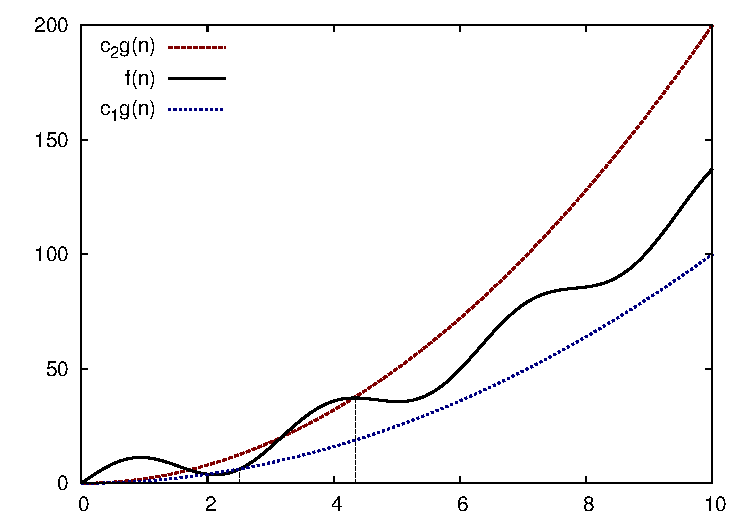
\includegraphics[width=.6\textwidth]{plot-3}
	\caption{Notazione asintotica \(\Theta\).}
	\label{fig:plot-3}
\end{figure}

\section{Complessità di un algoritmo e di un problema}

\begin{definition*}[complessità in tempo di un \alert{algoritmo}]
La più grande quantità di tempo richiesta \emph{per un input} di dimensione \(n\).
\end{definition*}
\begin{itemize}
	\item \(\Omicron(f(n))\): per tutti gli input, l'algoritmo costa al più \(f(n)\);
	\item \(\Omega(f(n))\): per tutti gli input, l'algoritmo costa almeno \(f(n)\);
	\item \(\Theta[f(n)]\): l'algoritmo richiede \(\Theta[f(n)]\) per tutti gli input.
\end{itemize}

\begin{definition*}[complessità in tempo di un \alert{problema computazionale}]
La complessità in tempo relativa \emph{a tutte le possibili soluzioni}.
\end{definition*}
\begin{itemize}
	\item \(\Omicron(f(n))\): complessità del miglior algoritmo che risolve il problema;
	\item \mbox{\(\Omega(f(n))\): dimostrare che nessun algoritmo può risolvere il problema in tempo inferiore a \(\Omega(f(n))\)};
	\item \(\Theta[f(n)]\): abbiamo trovato l'algoritmo ottimo.
\end{itemize}

\clearpage
\section{Esercizi}

\subsubsection*{Primo esercizio}

Iniziamo con degli esercizi banali che ci permetteranno di introdurre delle tecniche che utilizzeremo con le ricorrenze.
In particolare ci serviranno a renderci conto che non stiamo dimostrando equazioni, ma disequazioni.

\exercise{\( f(n) = 10 n^3 + 2 n^2 + 7 \overset{?}{=} \mathcal{O}(n^3) \)}

\textbf{Limite superiore}: Dobbiamo dimostrare che \( \exists c > 0, \exists m \geqslant 0: f(n) \bs{\leqslant} cn^3, \forall n \geqslant m\)
\[
\begin{WithArrows}
	f(n) &= 10 n^3 + 2 n^2 + 7 \Arrow[jump = 2]{\( \forall n \geqslant 1 \)} \\
	&\leqslant 10 n^3 + 2 n^{3} + 7 \\
	&\leqslant 10 n^3 + 2 n^3 + 7 n^3 \Arrow{sommiamo i termini} \\
	&= 19 n^3 \Arrow[tikz={text width=4cm}]{esiste una certa costante \(c\) per la quale \(f(n) \leqslant cn^3\) ?}\\
	&\overset{?}{\leqslant} cn^3 \Arrow{metto a confronto}\\
	19 n^3 &\leqslant cn^3 \Arrow{semplifico}\\
	19 \cancel{n^3} &\leqslant c\cancel{n^3}
\end{WithArrows}
\]

che è vera per ogni \(c \geqslant 19\) (abbiamo così trovato la costante moltiplicativa) e per ogni \(n \geqslant 1\) (introdotta nei calcoli), quindi \(m = 1\) (che deriva da \(\forall n \geqslant m\)).

\begin{figure}[H]\centering
	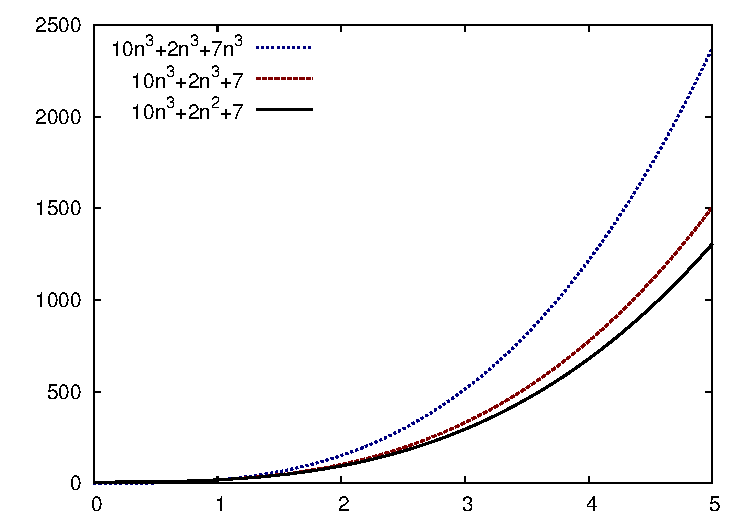
\includegraphics[width=.6\textwidth]{plot-0}
	\caption[]{Risoluzione grafica dell'esercizio.}
	\label{fig:plot-0}
\end{figure}

\begin{note}
In generale noi considereremo solo valori di \(n\) positivi, in quanto le funzioni di costo sono definite sull'insieme dei numeri naturali, non ha alcun senso definire una funzione di costo su una dimensione dell'input negativa.
\end{note}

\clearpage
\subsubsection*{Soluzione alternativa all'esercizio precedente}

Dato lo stesso esercizio posso esserci passaggi risolutivi diversi.
Risolviamo quindi l'esercizio precedente in modo diverso.

\exercise{\( f(n) = 10 n^3 + 2 n^2 + 7 \overset{?}{=} \mathcal{O}(n^3) \)}

\textbf{Limite superiore}: Dobbiamo dimostrare che \( \exists c > 0, \exists m \geqslant 0: f(n) \bs{\leqslant} cn^3, \forall n \geqslant m\)
\[
\begin{WithArrows}
	f(n) &= 10 n^3 + 2 n^2 + 7 \Arrow{\( \forall n \geqslant 1 \)} \\
	&\leqslant 10 n^3 + 2 n^{3} + 7 \Arrow{\(\forall n \geqslant \sqrt[3]{7}\)} \\
	&\leqslant 10 n^3 + 2 n^3 + n^3 \Arrow{sommiamo i termini} \\
	&= 13 n^3 \Arrow[tikz={text width=4cm}]{esiste una certa costante \(c\) per la quale \(f(n) \leqslant cn^3\) ?}\\
	&\overset{?}{\leqslant} cn^3 \Arrow{metto a confronto}\\
	13 n^3 &\leqslant cn^3 \Arrow{semplifico}\\
	13 \cancel{n^3} &\leqslant c\cancel{n^3}
\end{WithArrows}
\]
che è vera per ogni \( c \geqslant 13 \) e per ogni \( n \geqslant \sqrt[3]{7} \) (ad esempio con \(n=2\) abbiamo \(n^3 = 2^3 = 8\) che soddisfa la nostra condizione), quindi usiamo \( m = 2 \) (abbiamo semplificato, sarebbe \(m = \sqrt[3]{7}\), ma possiamo prendere un qualunque valore si trovi dopo \(n\) in modo totalmente arbitrario).

\begin{figure}[H]\centering
	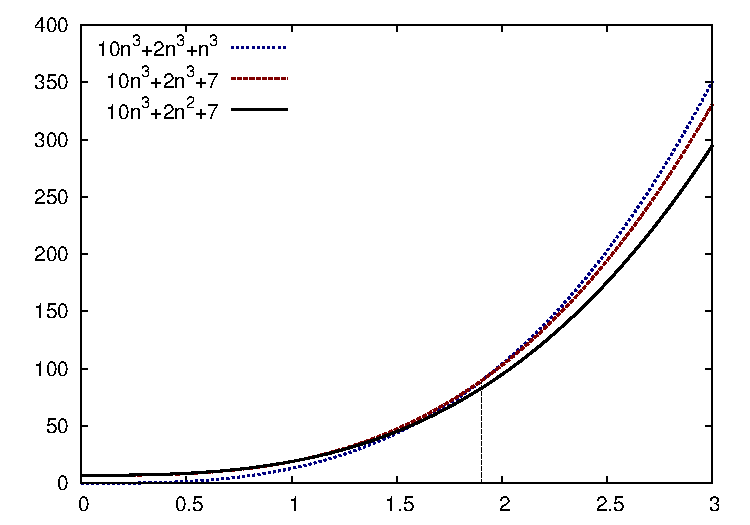
\includegraphics[width=.6\textwidth]{plot-0bis}
	\caption[]{Risoluzione grafica dell'esercizio.}
	\label{fig:plot-0bis}
\end{figure}

\clearpage
\subsubsection*{Secondo esercizio}

\exercise{\( f(n) = 3 n^2 + 7n \overset{?}{=} \Theta(n^2) \)}

\textbf{Limite inferiore}: Dobbiamo dimostrare che
\( \exists c_1 > 0, \exists m_1 \geqslant 0: \alert{f(n) \bs{\geqslant} c_1 n^2}, \forall n \geqslant m_1 \)
\[
\begin{WithArrows}
	f(n) &= 3 n^2 + 7 n \Arrow{\( \forall n \geqslant 0 \)} \\
	&\geqslant 3 n^2 \Arrow[tikz={text width=4cm}]{esiste una certa costante \(c\) per la quale \(f(n) \leqslant c_1 n^2\) ?}\\
	&\overset{?}{\geqslant} c_1 n^2 \Arrow{metto a confronto}\\
	3 n^2 &\leqslant c_1 n^2 \Arrow{semplifico}\\
	3 \cancel{n^2} &\leqslant c_1 \cancel{n^2}
\end{WithArrows}
\]
che è vera per ogni \( c_1 \bs{\leqslant} 3 \) e per ogni \( n \geqslant 0 \) (introdotta nei calcoli), quindi \( m_1 = 0 \).

\begin{note}
Abbiamo dimostrato quindi che \(f(n) = \Omega(n^2)\).
\end{note}

\textbf{Limite superiore}: Dobbiamo dimostrare che
\( \exists c_2 > 0, \exists m_2 \geqslant 0: \alert{f(n) \bs{\leqslant} c_2 n^2}, \forall n \geqslant m_2 \)
\[\begin{WithArrows}
	f(n) &= 3 n^2 + 2 n^2 + 7 n \Arrow{\( \forall n \geqslant 1 \)} \\
	&\leqslant 3 n^2 + 7 n^2 \Arrow{raccogliamo} \\
	&\leqslant 10 n^2 \Arrow[tikz={text width=4cm}]{esiste una certa costante \(c\) per la quale \(f(n) \leqslant c_2 n^2\) ?}\\
	&\overset{?}{\leqslant} c_2 n^2 \Arrow{metto a confronto}\\
	10 n^2 &\leqslant c_2 n^2 \Arrow{semplifico}\\
	10 \cancel{n^2} &\leqslant c_2 \cancel{n^2}
\end{WithArrows}\]
che è vera per ogni \( c_2 \bs{\geqslant} 10 \) e per ogni \( n \geqslant 1 \), %\\
quindi \( m_2 = 1 \).

\begin{note}
Abbiamo dimostrato quindi che \(f(n) = \mathcal{O}(n^2)\).
\end{note}

\textbf{Notazione \(\Theta\)}: \( \exists c_1 > 0, \exists c_2 > 0, \exists m \geqslant 0 \colon \alert{c_1 n^2 \bs{\leqslant} f(n) \bs{\leqslant} c_2 n^2}, \forall n \geqslant m \).

Con questi paramentri:
\begin{itemize}
	\item \(c_1 = 3\);
	\item \(c_1 = 10\);
	\item \(m = max\{m_1, m_2\} = max\{0, 1\} = 1\), ossia un valore dopo il quale la nostra proprietà è provata.
\end{itemize}

\begin{note}
Abbiamo dimostrato quindi che \(f(n) = \Theta(n^2)\).
\end{note}

\begin{figure}[H]\centering
	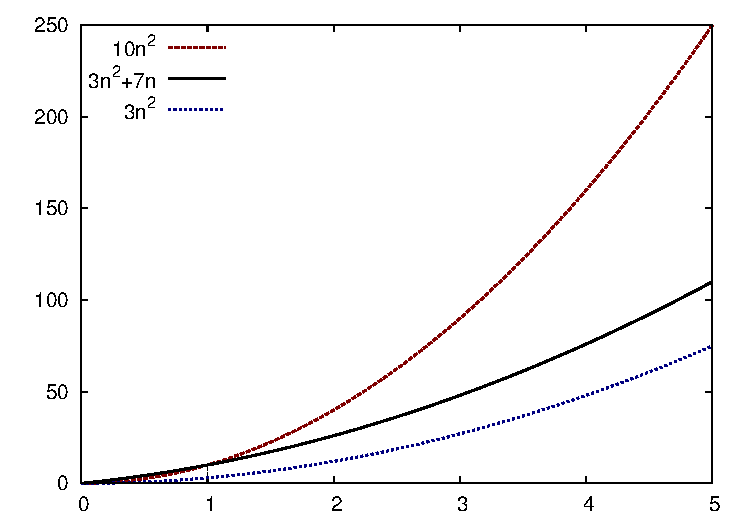
\includegraphics[width=.6\textwidth]{plot-1}
	\caption[]{Risoluzione grafica dell'esercizio.}
	\label{fig:plot-1}
\end{figure}

\clearpage
\section*{Errori comuni durante la risoluzione degli esercizi}

\subsubsection*{Dimostrare un limite superiore inesistente}

\exercise{\( f(n) = n^2 \overset{?}{=} \Omicron(n) \)}

\textbf{Limite superiore}: Dobbiamo dimostrare che \( \exists c > 0, \exists m \geqslant 0 \colon \alert{n^2 \bs{\geqslant} cn}, \forall n \geqslant m \).

Otteniamo che \(n^2 \leqslant cn \Leftrightarrow c \geqslant n\) (ad esempio con \(n=2\), \(2^2 \leqslant c \cdot 2 \Leftrightarrow c \geqslant 2\)), questo significa che \(c\) cresce con il crescere di \(n\), non possiamo quindi scegliere una \emph{costante} \(c\) che verifichi la proprietà.

\begin{figure}[H]\centering
	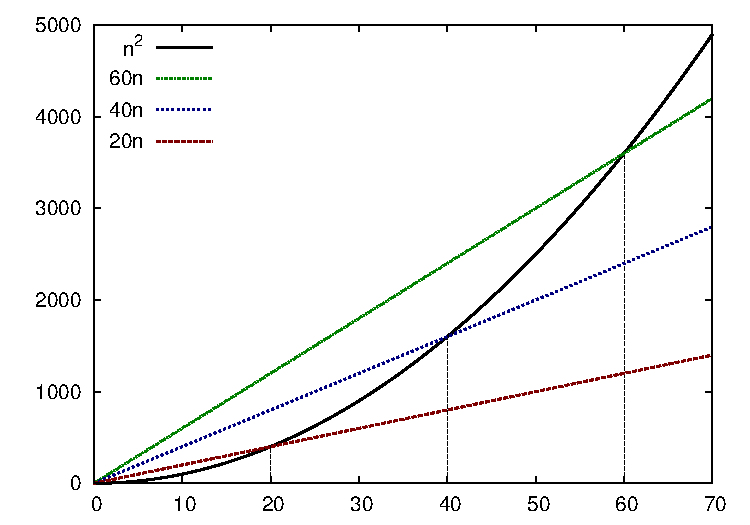
\includegraphics[width=.6\textwidth]{plot-nvsn2}
	\caption[]{Per qualunque fattore \(c\) scelto (ossia la pendenza della retta) la curva quadratica crescerà sempre più velocemente da un certo punto in poi.}
	\label{fig:plot-nvsn2}
\end{figure}

\subsubsection*{Dimostrare un limite inferiore inesistente}

\exercise{\( f(n) = n^2 \overset{?}{=} \Omega(n^3) \)}

\textbf{Limite inferiore}: Dobbiamo dimostrare che \(\exists c > 0, \exists m \geqslant 0, n^2 \geqslant cn^3, \forall n \geqslant m\).

Otteniamo che \(n^2 \geqslant cn^3 \Leftrightarrow c \leqslant \frac{1}{n}\) (ad esempio con \(n=2\), \(2^2 \geqslant c \cdot 2 \Leftrightarrow c \leqslant \frac{1}{2}\)), questo significa che \(c\) diminuisce al crescere di \(n\), non possiamo quindi scegliere una costante \(c\) che verifichi la proprietà.

\clearpage
\section{Complessità degli algoritmi e dei problemi a confronto}

In questa sezione ragioneremo su alcuni algoritmi risolutivi che ci sono stati insegnati, in alcuni casi si può migliorare la complessità, in altri è impossibile fare di meglio.

\begin{quote}
Qual è il rapporto fra un problema computazionale e l'algoritmo?
\end{quote}

\subsection{Moltiplicare numeri complessi}

La moltiplicazione fra numeri complessi avviene nel seguente modo: \((a + bi)(c + di) = [ac - db] + [ad + bc]i\).
Abbiamo in input \(a\), \(b\), \(c\), \(d\) e dobbiamo restituire in output \(ac - bd\) e \(ad + bc\).

Consideriamo un modello di calcolo dove la moltiplicazione costa \num{1} e le addizioni e sottrazioni costano \num{0.01}.
\begin{enumerate}
	\item Quanto costa l'algoritmo dettato dalla definizione?
	\item Riesci a fare meglio di così?
	\item Qual è il ruolo del modello di calcolo?
\end{enumerate}

L'algoritmo banale dettato dalla definizione costa \num{4.02}, in quanto bisogna fare 4 moltiplicazioni, 1 somma ed una sottrazione.

\subsubsection*{Soluzione di Gauss per la moltipicazione di numeri complessi}

La seguente è la soluzione di Gauss al problema, datata 1805.

Input: \(a\), \(b\), \(c\), \(d\), Output: \(A1 = ac - bd\), \(A2 = ad + bc\)
\let\oldtimes\times
\renewcommand\times{\mathcolor{red}{\bs{\oldtimes}}}
\let\oldplus\plus
\renewcommand\plus{\mathcolor{red}{\bs{\oldplus}}}
\let\oldminus\minus
\renewcommand\minus{\mathcolor{red}{\bs{\oldminus}}}
\[\begin{WithArrows}
m_1	&= a \times c \Arrow[tikz=-, jump=2, tikz=darker]{calcolo i valori intermedi} \\
m_2 &= b \times d \\
A_1 &= m_1 \minus m_2 \\
m_3	&= (a \plus b) \times (c \plus d) = ac + ad + bc + bd \Arrow{evito una moltiplicazione} \\
A_2	&= m_3 \minus m_1 \minus m_2 = ad + bc
\end{WithArrows}\]
\renewcommand\times{\oldtimes}
\renewcommand\plus{\oldplus}
\renewcommand\minus{\oldminus}

Il costo totale è \num{3.05}.

\begin{quote}
Si può fare ancora meglio di così?
Oppure è possibile dimostrare che non si può?
\end{quote}

\clearpage
\subsection{Sommare numeri binari}

\begin{note}
In questo caso usiamo il criterio del costo logaritmico.
\end{note}

L'algoritmo elementare della somma richiede di esaminare tutti gli \(n\) bit, il costo totale risulta \(cn\), dove \(c\) è il costo per sommare due bit e generare il riporto.

\begin{quote}
Esiste un metodo più efficiente?
\end{quote}

\`{E} dimostrabile per assurdo che \emph{non è possibile fare di meglio} di una soluzione lineare, poiché non è possibile sommare due numeri binari senza esaminare tutti gli \(n\) bit.

\subsection*{Limiti alla complessità di un problema}

\begin{definition*}[limite superiore, \(\mathcal{O}(f(n))\)]
Un problema ha complessità \(\mathcal{O}(f(n))\) \emph{se esiste almeno un algoritmo} che ha complessità \(\mathcal{O}(f(n))\).
\end{definition*}

\begin{note}
Il problema della somma dei numeri binari ha complessità \(\Omicron(n)\).
\end{note}

\begin{definition*}[limite inferiore, \(\Omega(f(n))\)]
Un problema ha complessità \(\Omega(f(n))\) \emph{se tutti i possibili algoritmi} che lo risolvono hanno complessità \(\Omega(f(n))\).
\end{definition*}

\begin{note}
Il problema della somma dei numeri binari ha complessità \(\Omega(n)\).
\end{note}

\subsection{Moltiplicare numeri binari}

L'algoritmo elementare del prodotto richiede di moltiplicare ogni bit con ogni altro bit, per un costo totale di \(c n^2\).

\begin{figure}[H]
	\centering
	\label{fig:mul}
	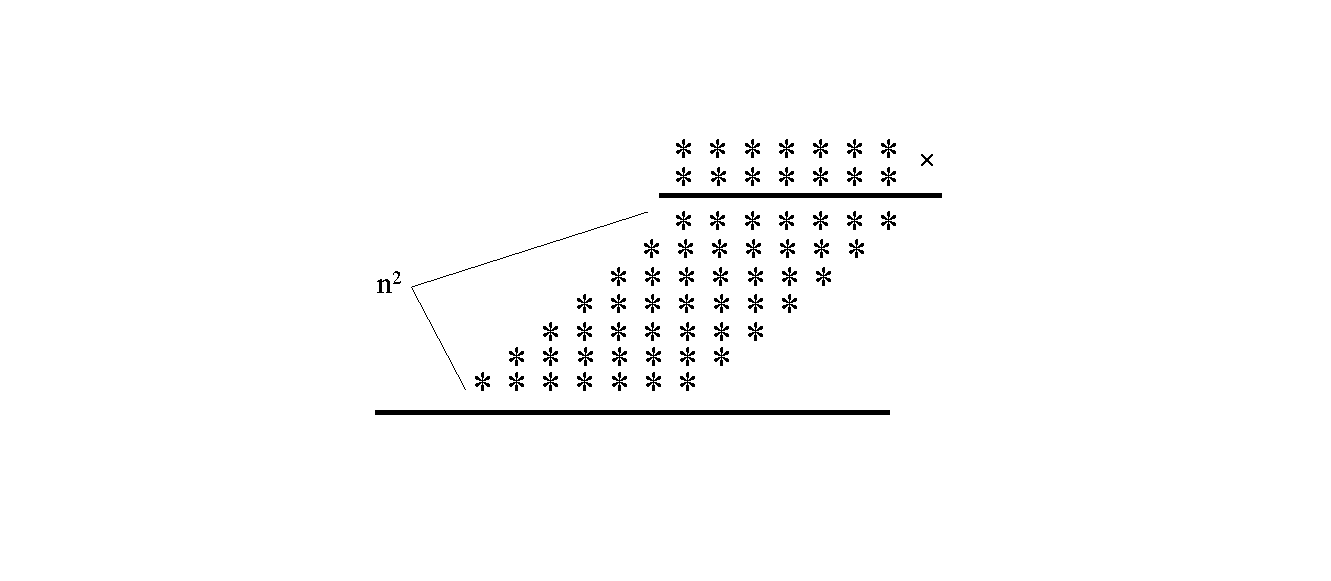
\includegraphics[width=.4\textwidth]{mul}
	\caption[]{Moltiplicazione di due numeri binari.}
\end{figure}

Si potrebbe concludere che il problema della moltiplicazione è molto più costoso del problema dell'addizione: ne è conferma la nostra esperienza.

\begin{note}
Per provare che il problema del prodotto è più costoso del problema della somma, dobbiamo provare che non esiste una soluzione in tempo lineare al problema del prodotto.
\end{note}

Abbiamo infatti erroneamente confrontato gli algoritmi, non i problemi!
Sappiamo solo che l'algoritmo della somma che ci hanno insegnato è più efficiente di quello della moltiplicazione.

Nel 1960, Kolmogorov enunciò che la moltiplicazione avesse limite inferiore pari a \(\Omega(n^2)\), una settimana dopo un suo studente Karatsuba riuscì a provare il contrario.
Osserviamo la sua soluzione.

\clearpage
\subsubsection*{Approccio divide-et-impera}

Karatsuba adottò un approccio divide-et-impera.

\begin{definition}[approccio divide-et-impera]
Si svolge in tre parti:
\begin{itemize}
	\item \textbf{Divide}: dividi il problema in sottoproblemi di dimensione inferiore;
	\item \textbf{Impera}: risolvi i sottoproblemi in maniera ricorsiva;
	\item (\textbf{Combina}): unisci le soluzioni dei sottoproblemi in modo da ottenere la risposta del problema principale.
\end{itemize}
\end{definition}
\[\begin{WithArrows}
X  &= a \cdot 2^{\nicefrac{n}{2}} + b \\
Y  &= c \cdot 2^{\nicefrac{n}{2}} + d \\
XY &= ac \cdot 2^n + (ad + bc) \cdot 2^{\nicefrac{n}{2}} + db
\end{WithArrows}\]

\begin{algorithm}[H]
\caption{Moltiplicazione di due numeri binari}

\BlankLine
% \tcp{moltiplica due numeri binari}
\prototype{\Array{\Bool} \pdi{\Array{\Bool} X, \Array{\Bool} Y, \Int n}}{
\params{X}[numero binario]
\params{Y}[numero binario]
\params{n}[numero di bit contenuti]

	\BlankLine
	\eIf{\(n \Equal 1\)}{
		\Return \(X[1] \cdot Y[1]\)\Comment*[l]{eseguo la moltiplicazione di due bit}
	}{
		spezza \(X\) in \(a\);\(b\) e \(Y\) in \(c\);\(d\)\;
		\Return \(\pdi{a, c, \nicefrac{n}{2}} \cdot 2^n + (\pdi{a, d, \nicefrac{n}{2}} + \pdi{b, c, \nicefrac{n}{2}}) \cdot 2^{\nicefrac{n}{2}} + \pdi{b, d, \nicefrac{n}{2}}\)\;
	}
}
\end{algorithm}

\paragraph{Complessità}
Moltiplicare per \(2^t\) è equivalente ad eseguire uno \foreign{shift} di \(t\) posizioni, in tempo lineare, quindi l'equazione di ricorrenza risultante è
\[
	T(n) =
	\begin{dcases}
		c_1                               & n = 1 \\
		4T(\nicefrac{n}{2}) + c_2 \cdot n & n > 1 \\
	\end{dcases}
	% = \mathcal{O}(n^2)
\]

\begin{note}
Non sappiamo ancora trattare questo genere di problemi, quindi facciamo solo degli accenni.
\end{note}

\paragraph{Analisi della ricorsione}
% (vedi figura) % TODO inserire immagine ricorsione
Al primo passo la chiamata ricorsiva avviene su una dimesione \(n\), al secondo passo vengono effettuate \(4\) chiamate ricorsive su una dimesione \(\nicefrac{n}{2}\), al terzo passo vengono effettuate \(4^2 = 16\) chiamate ricorsive su una dimesione \(\nicefrac{n}{2^2}\)\dots
al livello \(i\)-esimo vengono effettuate \(4^i\) chiamate ricorsive su una dimesione \(\nicefrac{n}{2^i}\).
Una volta arrivati al passo \(\log_2 n\) vengono effettuate \(4^{\log n}\) chiamate ricorsive su una dimesione pari al caso base \(T(1)\), per la proprietà dei logaritmi \(4^{\log n} = n^{\log 4} = n^2\), le dimensioni delle chiamate ricorsive vengono ridotte ad una semplice costante.
Possiamo quindi concludere che \(T(n) = \Omicron(n^2)\).

\clearpage
\subsubsection*{Moltiplicazione di Karatsuba}

\`{E} possibile ridurre ulteriormente la complessità.
\[\begin{WithArrows}
	A_1 &= a \times c \Arrow[jump=2, tikz=darker]{calcolo un valore intermedio} \\
	A_2 &= b \times d \\
	m   &= (a \plus b) \times (c \plus d) = ac + ad + bc + bd \Arrow{evito una moltiplicazione} \\
	A_3 &= m \minus A_1 \minus A_2 = ad + bc
\end{WithArrows}\]

\paragraph{Principio}
Effettuo un'unica moltiplicazione che mi permette di calcolare un valore intermedio che contiene la somma di tutte le combinazioni (\(m\)), e ricavo \(ad + bc\) tramite due sottrazioni (nello stesso modo in cui lavorava Gauss) evitando così una moltiplicazione.

\begin{algorithm}[H]
\caption{Moltiplicazione di Karatsuba}

\BlankLine
\prototype{\Array{\Bool} \karatsuba{\Array{\Bool} X, \Array{\Bool} Y, \Int n}}{

	\BlankLine
	\eIf{\(n \Equal 1\)}{
		\Return \(X[1] \cdot Y[1]\)\Comment*[l]{rimane invariato}
	}{
		spezza \(X\) in \(a\);\(b\) e \(Y\) in \(c\);\(d\)\;

		\BlankLine
		\Array{\Bool} \(A1 = \karatsuba{a, c, \nicefrac{n}{2}}\)\;
		\Array{\Bool} \(A3 = \karatsuba{b, d, \nicefrac{n}{2}}\)\;
		\Array{\Bool} \(m\) = \karatsuba{\(a + b\), \(c + d\), \(\nicefrac{n}{2}\)}\Comment*[l]{potrebbe essere \(\nicefrac{n}{2} + 1\)}
		\Array{\Bool} \(A2 = m - A1 - A3\)\Comment*[l]{ottengo A2 tramite sottrazione}

		\BlankLine
		\Return \(A1 \cdot 2^n + A2 \cdot 2^{\nicefrac{n}{2}} + A3\)\Comment*[l]{effettuo degli shift}
	}
}
\end{algorithm}

\paragraph{Complessità}
L'equazione di ricorrenza risultante è:
\[
	T(n) =
	\begin{dcases}
		c_1                               & n = 1 \\
		3T(\nicefrac{n}{2}) + c_2 \cdot n & n > 1 \\
	\end{dcases}
	% = \mathcal{O}(n^{1.58\dots})
\]

\paragraph{Analisi della ricorsione}
% TODO inserire immagine Ricorsione
Al primo passo la chiamata ricorsiva avviene su una dimesione \(n\), al secondo passo vengono effettuate \(3\) chiamate ricorsive su una dimesione \(\nicefrac{n}{2}\), al terzo passo vengono effettuate \(3^2 = 9\) chiamate ricorsive su una dimesione \(\nicefrac{n}{3^2}\)\dots
al livello \(i\)-esimo vengono effettuate \(3^i\) chiamate ricorsive su una dimesione \(\nicefrac{n}{2^i}\).
Una volta arrivati al passo \(\log_2 n\) vengono effettuate \(3^{\log n}\) chiamate ricorsive su una dimesione pari al caso base \(T(1)\), per la proprietà dei logaritmi \(3^{\log n} = n^{\log 3} = n^{1.58\dots}\).
Le dimensioni delle chiamate ricorsive vengono ridotte ad una semplice costante.
Possiamo quindi concludere che \(T(n) = \Omicron(n^{1.58\dots})\).

\begin{note}
L'algoritmo ingenuo (\foreign{na\"if}) non è sempre il migliore a meno che non sia possibile dimostrare il contrario.
\end{note}

Negli anni sono stati proposti diversi algoritmi, che il limite inferiore al problema della moltiplicazione sia \(\Omega(n \log n)\) è una congettura.
Una congettura è un'affermazione o un giudizio fondato sull'intuito, ritenuto probabilmente vero, ma non ancora rigorosamente dimostrato, cioè dunque relegato solamente a rango di ipotesi.

Nella GNU Multiple Precision Arithmetic Library vengono utilizzati diversi algoritmi al crescere di \(n\), il valore soglia per cui si predilige un algoritmo rispetto ad un altro dipende dal tipo di architettura.

\clearpage
\section{Algoritmi di ordinamento}

In questa lezione impareremo a capire quando è meglio utilizzare un algoritmo di ordinamento rispetto ad un altro.

In alcuni casi, gli algoritmi si comportano diversamente a seconda delle caratteristiche dell'input.
Conoscere in anticipo tali caratteristiche permette di scegliere l'algoritmo migliore in quella determinata situazione.

\section*{Tipologia di analisi}

Esistono tre tipi di analisi:
\begin{enumerate}
	\item analisi del \textbf{caso pessimo}: è la tipologia più importante, il tempo di esecuzione nel caso peggiore è il limite superiore al tempo di esecuzione per qualsiasi input. Per alcuni algoritmi il caso peggiore si verifica molto spesso (ad esempio nella ricerca di dati non presenti nel database);
	\item analisi del \textbf{caso medio}: è difficile da definire (cosa si intende per \enquote{medio} ?), dobbiamo avere una conoscenza pregressa sulle distribuzioni;
	\item analisi del \textbf{caso ottimo}: può avere senso se si conoscono informazioni particolari sull'input.
\end{enumerate}

\section*{Problema dell'ordinamento}

Data una sequenza \(A = a_1, a_2, \dots, a_n\) di \(n\) valori in input, il problema dell'ordinamento consiste nel restituire in output una sequenza \(B = b_1, b_2, \dots, b_n\) che sia una permutazione di \(A\), tale per cui \mbox{\(b_1 \leqslant b_2 \leqslant \dots \leqslant b_n\)} (ovvero che ci sia un ordinamento \emph{totale}).

Un approccio \enquote{demente} è quello di generare tutte le possibili permutazioni (complessità \(n!\)) fino a quando non se ne trova una ordinata.

\clearpage
\subsection{Selection sort}

Un approccio banale (\foreign{na\"if}) è quello di cercare il minimo e metterlo nella posizione corretta, riducendo il problema agli \(n-1\) valori rimanenti.

\begin{algorithm}[H]
	\caption{selectionSort}
	%&../preamble

\setcounter{section}{1}
% \setcounter{algocf}{5}

% arara: pdflatex: { synctex: no }
% arara: latexmk: { clean: partial }
\ifstandalone
\begin{document}
\begin{algorithm}[H]
\fi

\tcp{effettua l'ordinamento di un vettore}
\prototype{\selectionSort{\Array{\Item} A, \Int n}}{
	\From(\tcp*[h]{l'ultimo elemento è ordinato}){\Int \(i \Assign 1\) \DownTo \(n-1\)}{
		\Int \(j \Assign \minFunction{A, i, n}\)\Comment*[l]{ricerca il nuovo minimo}
		% \Swap{\(A[i]\)}{\(A[j]\)}\Comment*[l]{lo metto nella posizione corretta}
		\(A[i] \leftrightarrow A[j]\)\Comment*[l]{lo metto nella posizione corretta}
	}
}

\BlankLine
\tcp{cerca l'indice dell'elemento più piccolo}
\prototype{\Int \minFunction{\Array{\Item} A, \Int i, \Int j}}{

	\BlankLine
	\Int \(min \Assign i\) \Comment*[h]{posizione del minimo parziale}\;
	\From{\Int \(j \Assign i+1\) \DownTo \(n\)}{

		\BlankLine
		\If(\Comment*[h]{ho trovato un nuovo minimo}){\( A[j] < A[min] \)}{
			\(min \Assign j\) \Comment*[h]{nuovo minimo parziale}\;
		}
	}

	\BlankLine
	\Return \(min\)\Comment*[l]{restituisco l'indice dell'elemento più piccolo}
}
% \begin{algomathdisplay}
% 	\sum_{i=1}^{n-1} (n-1) = \sum_{i=1}^{n-1} i = \frac{n(n-1)}{2} = n^2 - \frac{n}{2} = \Theta(n^2)
% \end{algomathdisplay}
\ifstandalone
\end{algorithm}
\end{document}
\fi

\end{algorithm}

\begin{figure}[H]\centering
	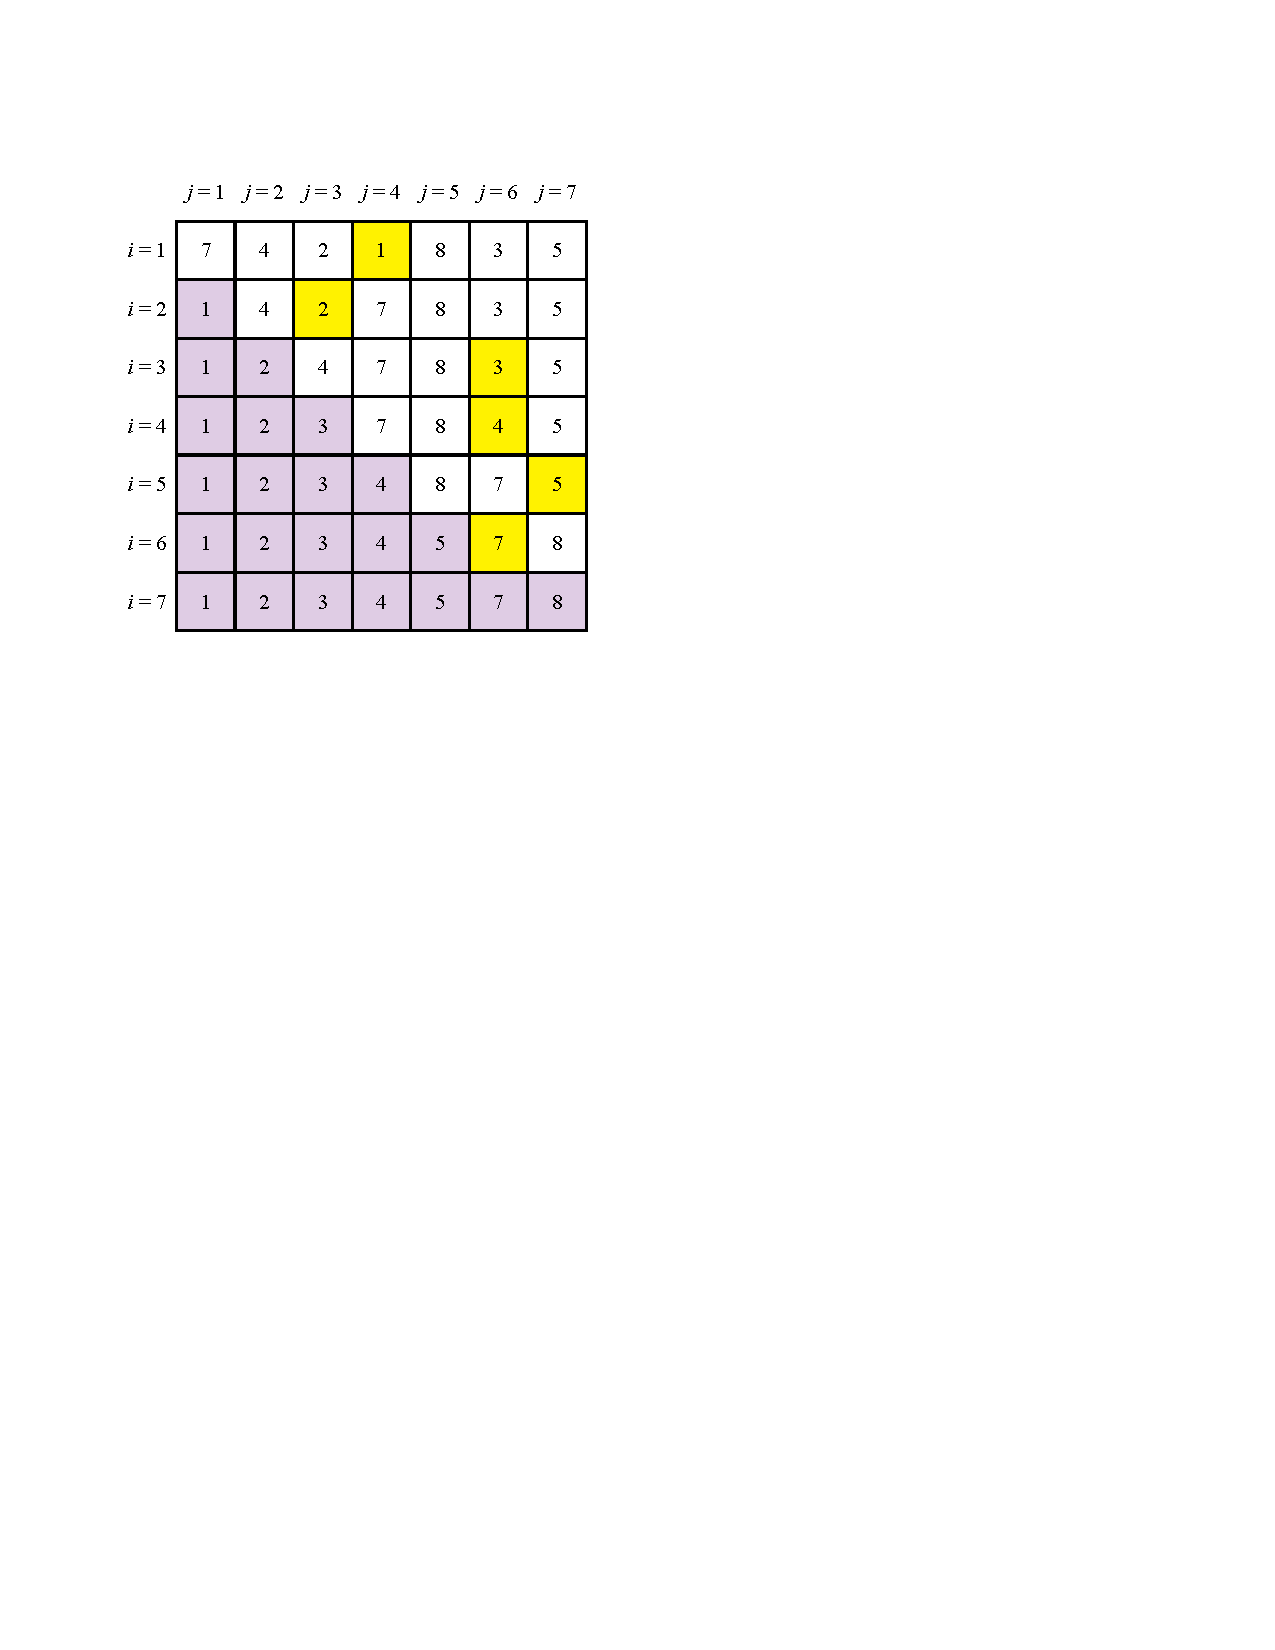
\includegraphics{selection}
	\caption[]{Funzinamento dell'algoritmo \selectionSort.}
\end{figure}

% TODO scrivere spiegazione selectionSort
% \paragraph{Spiegazione}
% Diamo per scontato che il primo elemento sia ordinato.

\begin{hint}
Provalo su carta!
Un algoritmo dev'essere provato per essere capito!
\end{hint}

\paragraph{Analisi della complessità}
Il ciclo effettua \(n\) chiamate della funzione \minFunction (una per ciascuna iterazione).
Ad ogni iterazione il vettore su cui viene calcolato il minimo risulta più piccolo di un elemento.
\[\begin{WithArrows}
	&\sum_{i=1}^{n-1} (n-1) \Arrow{\(10+9+\dots+1 \Leftrightarrow 1+2+\dots+10\)} \\
	&= \sum_{i=1}^{n-1} i \\
	&= \frac{n(n-1)}{2} \Arrow{svolgo i calcoli} \\
	&= n^2 - \frac{n}{2} \\
	&= \Theta(n^2)
\end{WithArrows}\]
Posso dire che è \(\Theta(n^2)\), e non solo che \(\Omega(n^2)\), perché indipendentemente dall'ordine iniziale ci metterà sempre lo stesso tempo.
In altre parole, il caso migliore, peggiore e medio coincidono.

\clearpage
\subsection{Insertion sort}

Un algoritmo che si basa sul principio di ordinamento di una \enquote{mano} di carte da gioco è il seguente:

\begin{algorithm}[H]
	\caption{insertionSort}
	%&../preamble

% arara: pdflatex: { synctex: no }
% arara: latexmk: { clean: partial }
\ifstandalone
\begin{document}
\begin{algorithm}[H]
\fi

% \tcp{efficiente per ordinare piccoli insiemi di elementi}
\tcp{effettua l'ordinamento di un vettore}
\prototype{\insertionSort{\Item{} A, \Int n}}{

	\BlankLine
	\From(\Comment*[h]{il 1\textsuperscript{o} elemento verrà ordinato in seguito}){\Int \(i=2\) \DownTo \(n\)}{

		\BlankLine
		\Item \(temp \Assign A[i]\) \Comment*[h]{elemento da ordinare}\;
		\Int \(j \Assign i\)\;

		\BlankLine
		\While{\(j > 1\) \And \(A[j-1] > temp\)}{
			\(A[j] \Assign A[j-1]\) \Comment*[h]{copio l'elemento}\;
			\Decrement{j} \Comment*[h]{mi sposto}\;
		}

		\BlankLine
		\(A[j] \Assign temp\)\;
	}
}
% \tcp{vettore già ordinato: \(\Omega(n)\)}
% \tcp{vettore decrescente: \(\Omicron(n^2)\)}
% \tcp{in media \(\Omicron(n^2)\)}
\ifstandalone
\end{algorithm}
\end{document}
\fi

\end{algorithm}

% TODO scrivere spiegazione insertionSort
% \paragraph{Spiegazione}
% Diamo per scontato che il primo elemento sia ordinato.

Questo è un algoritmo molto efficiente per ordinare piccoli insiemi di elementi.

\paragraph{Analisi della complessità}
Il \emph{costo di esecuzione} di questo algoritmo non \emph{dipende} solo dalla dimensione del vettore, ma anche \emph{dalla distribuzione dei dati in ingresso}.
Nel caso in cui il vettore sia già \emph{ordinato} il costo è \(\Omicron(n)\), in quanto non si entra mai nel secondo ciclo dato che la condizione risulta falsa.
Nel caso in cui il vettore sia \emph{ordinato in ordine inverso} è \(\Omega(n^2)\).
In media (informalmente) possiamo assumere che metà dei valori sia ordinata rispetto la loro disposizione finale e quindi metà di loro dovrà fare \(n\) passi per arrivare alla destinazione per una complessità di \(n \cdot \nicefrac{n}{2} = \Omicron(n^2)\).

Infine quando sappiamo che i valori sono quasi ordinati o che \(n\) è molto piccolo (nell'ordine di 16 o 32 elementi) allora questo algoritmo risulta efficiente.

\clearpage
\subsection{Merge sort}

MergeSort è basato sulla tecnica divide-et-impera vista in precendenza.
Ma come la utilizza?

\begin{definition}[approccio divide-et-impera di MergeSort]
Si svolge in tre parti:
\begin{itemize}
	\item \textbf{divide}: spezza il vettore di \(n\) elementi in 2 sottovettori di \(\frac n 2\) elementi;
	\item \textbf{impera}: chiama \mergeSort ricorsivamente sui due sottovettori (ottenendo due metà ordinate);
	\item (\textbf{combina}): unisce (da questo deriva \foreign{merge}) le due sequenze ordinate.
\end{itemize}
\end{definition}

L'idea alla base di questo algoritmo sfrutta il fatto che è possibile \emph{unire due sottovettori ordinati} in un vettore ordinato \emph{in tempo lineare}.

\begin{algorithm}[H]
	\caption{mergeSort}
	%&../preamble

% arara: pdflatex: { synctex: no }
% arara: latexmk: { clean: partial }
\ifstandalone
\begin{document}
\begin{algorithm}[H]
\fi

\BlankLine
\tcp{ordina i sottovettori}
\prototype{\mergeSort{\Item{} \(A\), \Int \(primo\), \Int \(ultimo\)}}{

	\BlankLine
	\If(\Comment*[h]{devono esistere almeno due elementi}){\(primo < ultimo\)}{
		\Int \(mezzo \Assign \floor{\frac{primo + ultimo}{2}}\)\;
		\mergeSort{\(A\), \(primo\), \(mezzo\)}\;
		\mergeSort{\(A\), \(mezzo+1\), \(ultimo\)}\;
		\merge{\(A\), \(primo\), \(ultimo\), \(mezzo\)}\Comment*[l]{unisce le soluzioni}\;
	}
}

\ifstandalone
\end{algorithm}
\end{document}
\fi

% \BlankLine
% \BlankLine
% Equazione di ricorrenza:
% \[
% 	T =
% 	\begin{dcases}
% 		\Theta(1) & n = 1\\
% 		\T*{\nicefrac{n}{2}} + \T*{\nicefrac{n}{2}} + \Theta(n) & n > 1 \\
% 	\end{dcases}
% 	=
% 	\begin{dcases}
% 		c & n = 1\\
% 		2\T{\nicefrac{n}{2}} + dn & n > 1\\
% 	\end{dcases}
% \]
%
% \BlankLine
% Analisi per livelli:
% \[
% \Omicron \left( \sum_{i=0}^{k} \Ccancel{2^i} \frac{n}{\Ccancel{2^i}} \right) = \Omicron \left( \sum_{i=0}^{k} n \right) = \Omicron(k \cdot n) = \Omicron(n \log n)
% \]
% %
% Teorema dell'esperto:
%
% \begin{minipage}[t]{.4\linewidth}
% \begin{align*}
% 		\alpha &= \log_2 2 = 1 \\
% 		\beta  &= 1 \\
% 		\alpha &= \beta \\
% \end{align*}
% \end{minipage}
% \begin{minipage}[t]{.4\linewidth}
% \begin{align*}
% 	T &= \Omicron(n^{\alpha} \log n) \\
% 	  &= \Omicron(n \log n) \\
% \end{align*}
% \end{minipage}

	%&../preamble

% arara: pdflatex: { synctex: no }
% arara: latexmk: { clean: partial }
\ifstandalone
\begin{document}
\begin{algorithm}[H]
\fi

\BlankLine
\tcp{effettua l'ordinamento dei sotto-vettori}
\prototype{\merge{\Item \(A\), \Int \(primo\), \Int \(ultimo\), \Int \(mezzo\)}}{
	\Int \(i\), \(j\), \(k\), \(h\)\;

	\BlankLine
	\tcp{inizializzo i puntatori}
	\(i \Assign primo\)\;
	\(j \Assign mezzo\)\;
	\(k \Assign primo\)\tcp*[l]{\(k\): indica la prossima posizione di scrittura}

	\BlankLine
	% \tcp{}
	\While{\(i \leqslant mezzo\) \And \(j \leqslant ultimo\)}{

		\BlankLine
		\tcp{B è il vettore di appoggio in cui memorizzo la porzione di vettore già ordinata}
		\eIf{\(A[i] \leqslant A[j]\)}{
			\tcp{l'elemento è gia ordinato}
			\(B[k] \Assign A[i]\)\;
			\Increment{i}\;
		}{
			\(B[k] \Assign A[j]\)\;
			\Increment{j}\;
		}

		\BlankLine
		\tcp{\emph{in entrambi i casi} ho inserito un valore}
		\Increment{k}\;
	}

	\BlankLine
	\tcp{se uno dei due vettori finisce ricopio la parte ordinata alla fine del vettore d'appoggio}
	\(j \Assign ultimo\)\;
	\From{\(h \Assign mezzo\) \DownTo \(i\)}{
		\(A[j] \Assign A[h]\)\;
		\Decrement{j}\;
	}

	\BlankLine
	\tcp{ricopio il vettore d'appoggio del vettore originale}
	\From{\(j \Assign primo\) \DownTo \(k-1\)}{
		\(A[j] \Assign B[j]\)\;
	}
}

\ifstandalone
\end{algorithm}
\end{document}
\fi

\end{algorithm}

% TODO scrivere spiegazione mergeSort
% \paragraph{Spiegazione}
% Quando un'array diventa vuoto, copia tutti i valori dall'array rimanente nell'array ordinato.

\clearpage
\paragraph{Analisi della complessità}
Assumiamo (per semplicità) che \(n = 2^k\) (ovvero che l'altezza dell'albero di suddivisioni sia esattamente \(k = \log_2 n\)) e che tutti i sottovettori abbiano dimensioni che sono potenze esatte di 2.
L'equazione di ricorrenza risultante è la seguente:
\begin{align*}
	T &=
	\begin{dcases}
		\Theta(1) & n = 1\\
		\T*{\nicefrac{n}{2}} + \T*{\nicefrac{n}{2}} + \Theta(n) & n > 1 \\
	\end{dcases}\\
	&=
	\begin{dcases}
		c & n = 1\\
		2\T{\nicefrac{n}{2}} + dn & n > 1\\
	\end{dcases}\\
\end{align*}
Qual è il costo computazionale di \mergeSort?

\begin{figure}[H]\centering
	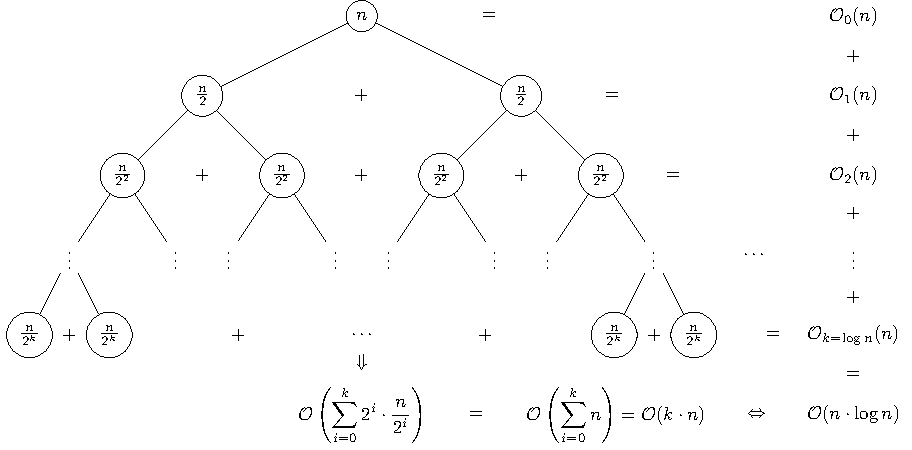
\includegraphics{mergesort-recursion}
	\caption[]{Analisi per livelli del costo di \mergeSort}
\end{figure}

L'analisi per livelli è la seguente:
\[\begin{WithArrows}
	&\Omicron \left( \sum_{i=0}^{k} \Ccancel{2^i} \frac{n}{\Ccancel{2^i}} \right) \Arrow{semplifico}\\
	&= \Omicron \left( \sum_{i=0}^{k} n \right) \Arrow{equivalente}\\
	&= \Omicron((k+1) \cdot n) \Arrow{\(k+1\) elementi, semplico perché è una costante}\\
	&= \Omicron(k \cdot n) \Arrow{\(k = \log n\)}\\
	&= \Omicron(n \log n)
\end{WithArrows}\]

\(\Omicron(n \log n)\) è asintoticamente migliore di \(\Omicron(n^2)\).
Questo algoritmo è preferibile --- per grandi dimensioni di \(n\) --- al \selectionSort e all'\insertionSort.

% NOTE fra dice che è abbastanza inutile 😞
% \section{Conclusioni}
%
% Abbiamo visto tre algoritmi di ordinamento:
% \begin{itemize}
% 	\item \selectionSort
% 	\item \insertionSort
% 	\item \mergeSort
% \end{itemize}
% Nell'ultima lezione vedremo molti altri algoritmi di ordinamento.
\ifsubfile
\end{document}
\fi
